\section{Data}

\subsection{Kilde, periode og labels}

Trafikkdata hentes fra Statens vegvesens åpne Traffic Data API, som inneholder
aggregerte registreringer fra offentlige veger \cite{vegvesen-traffic-portal}. Uttrekket
dekker 1. januar 2022 til 1. juli 2026 i lokal tid og gjelder feltet
\enquote{Totalt} ved punkt \texttt{14630V805616}. Den normaliserte timeaksen har
39 407 timer. Av disse har 38 956 observert trafikkvolum og 451 mangler verdi. Perioden
2022--2025 har 35 064 timer, 34 613 observasjoner og alle de 451 manglene. Den
reserverte perioden 2026 H1 har 4 343 observerte timer og ingen mangler.

Figur~\ref{fig:danmarks-plass-kart} gir geografisk kontekst for
registreringsområdet.

\begin{figure}[tbp]
  \centering
  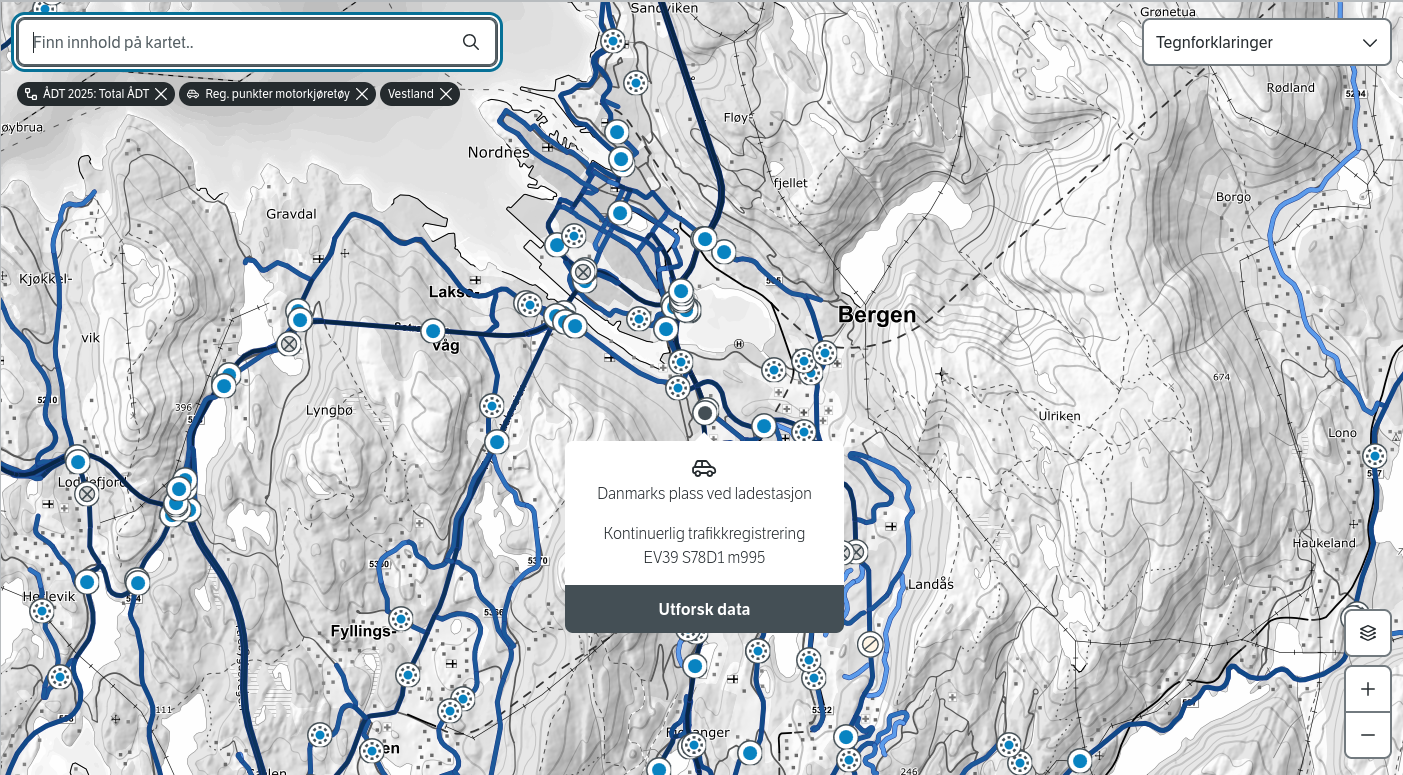
\includegraphics[width=0.94\textwidth]{figures/danmarks_plass.png}
  \caption{Geografisk oversikt over registreringsområdet ved Danmarks plass i
  Statens vegvesens Trafikkdataportal. Skjermbildet viser portalens kartvisning
  og valgte målested.}
  \label{fig:danmarks-plass-kart}
\end{figure}

Det opprinnelige API-uttrekket inneholder 39 025 rader. Kvalitetsrapporten markerer
69 av dem som ugyldige fordi volum mangler, men finner ingen dupliserte timestamps.
Når datasettet reindekseres til alle forventede UTC-timer, blir både disse radene og
timer uten API-rad stående som ukjente verdier. Forskjellen mellom rått radantall og
39 407 timer på den komplette aksen er derfor forventet og dokumentert, ikke et tap
som oppstår under behandling.

API-resultatet lagres først som rå CSV sammen med kilde, hentetidspunkt, punkt-ID,
periode og radantall. Det prosesserte datasettet får en sidecar-fil med SHA-256 for
råfilen, kvalitetsrapport og kolonneliste. Rådata, prosesserte data og
modellartefakter er utelatt fra Git, men kan gjenskapes med \texttt{make
build-app-model}. Denne kommandoen henter hele perioden, bygger datasettet og trener
sluttmodellen.

Labelen oppstår uten manuell annotering: for en feature-rad ved $t$ slås
\texttt{traffic\_volume} ved nøyaktig $t+1$ opp som
\texttt{target\_traffic}. Trafikkmåleren er dermed både datakilde og fasit. Dette gir
konsistente enheter, men ikke nødvendigvis en feilfri sannhet; sensorfeil og
ufullstendig dekning kan fortsatt påvirke både features og labels. API-ets
kvalitetsinformasjon lagres i rådataene, mens denne prosjektversjonen primært bruker
tilstedeværelse, gyldig timestamp og ikke-negativt volum som valideringskrav.

\subsection{Rensing og målegap}

Innlest tid konverteres til tidssonebevart UTC, sorteres og kontrolleres for ugyldige
og dupliserte tidspunkter. Kalenderinformasjon beregnes etter konvertering til
\texttt{Europe/Oslo}. Denne arbeidsdelingen bevarer entydige tidspunkt gjennom
sommertid og vintertid samtidig som time og dato får riktig lokal betydning.

Det finnes to dokumenterte målegap: 67 timer fra 4. juni 2022 kl. 21 til 7. juni
kl. 15, og 384 timer fra 2. oktober 2024 kl. 10 til 18. oktober kl. 09, alle tider i
\texttt{Europe/Oslo}. Pipelinen oppretter en komplett timeakse og lar disse 451
verdiene stå som manglende. De blir ikke satt til null, interpolert eller erstattet.
Null ville betydd observert fravær av trafikk, mens en manglende verdi betyr at
volumet er ukjent. Minimum og maksimum blant observerte timer i hele datasettet er
henholdsvis 40 og 4 235 kjøretøy; ingen observerte timer er null.

Den innledende EDA-en viste et tydelig døgn- og ukemønster. For 2022--2025 var
gjennomsnittet høyest kl. 15 med 3 426 kjøretøy per time og lavest kl. 03 med 185.
Helgesnittet var 1 275, som var 32,5 prosent lavere enn hverdagssnittet på 1 889.
Disse mønstrene begrunner kalenderfeatures og den ukentlige baselinen, men de brukes
ikke som en alternativ fasit. Volumfordelingen alene sier heller ikke om en høy verdi
er normal for en bestemt dato.

Alle lag og targets hentes ved eksakt timestamp, aldri ved radforskyvning. Hvis en
feature krever $t-24$ og denne timen ligger i et målegap, blir featuren manglende selv
om forrige tilgjengelige rad finnes 25 timer tilbake. Modellrader med manglende
nødvendig trafikklag eller target fjernes før trening og evaluering. Dette er et
dokumentert utvalg, ikke imputering, og hindrer at observasjoner flyttes over hull i
serien.

\subsection{Feature engineering}

Sluttmodellen bruker 14 features. Seks beskriver lokal kalender: time, ukedag,
måned, helg samt sinus og cosinus av time. Fem deterministiske indikatorer markerer
offentlig helligdag, dag før og etter helligdag, jul- og nyttårsperioden og 17. mai.
De tre numeriske traffic lag features er observert volum ved nøyaktig $t-24$, $t-48$ og
$t-168$. Alle er kjent eller kan konstateres som manglende ved prognosetidspunktet.
Den tree-based sluttmodellen krever ingen scaling.

Sinus og cosinus gjør at kl. 23 og kl. 00 ligger nær hverandre i
feature-representasjonen. Helligdagsindikatorene beregnes fra kalenderen og krever
ingen observerte fremtidsdata. Trafikklagene følger derimot absolutte tidsforskjeller
i UTC. Dermed endres ikke den faktiske avstanden ved overgang mellom sommer- og
vintertid, selv om det lokale klokkeslettet kan være annerledes.

Værdataene ble hentet fordi prosjektets opprinnelige hypotese var at weather features
kunne forbedre prediction utover det historisk trafikk alene ga. Historiske
observasjoner kom fra MET Norways Frost API for Bergen--Florida (SN50540). Frost gir
tilgang til arkiverte observasjoner og krever kilde,
referansetid og element i forespørselen \cite{frost-howto}. Temperatur og nedbør
dekket 35 016 av 35 064 timer i 2022--2025, mens vind dekket 34 458. Prosjektet
brukte konservative weather lag features fordi \texttt{referenceTime} beskriver
observasjonstid, ikke publiseringstid \cite{frost-time-concepts}. Både de direkte
weather lag features og en senere avledet weather feature-pakke ga svakere
validation enn traffic-only model. Det sentrale forsøket på å forbedre modellen med
vær lyktes dermed ikke, og Frost inngår derfor ikke i sluttmodellen eller appen.

\subsection{Personvern og etikk}

Datasettet inneholder aggregerte passeringstall per time, ikke kjøretøy- eller
personidentifikatorer. Personvernrisikoen er derfor lav. Den viktigste etiske
risikoen er feilaktig bruk: ett registreringspunkt representerer ikke all trafikk på
Danmarks plass eller Bergen, og en prognose kan være misvisende ved hendelser som
modellen ikke kjenner. Appen oppgir derfor punkt-ID, datakilde og begrensning. En
senere operativ løsning bør i tillegg dokumentere datalisens, tilgjengelighet,
sensorendringer og hvem som har ansvar for beslutninger som støttes av prognosen.
